%==============================================================================
%  FINAL PROJECT PAPER  (IEEE Conference format)  -- Category A
%  Efficient Regional ERA5 -> Zarr: storage + parallel data-loading trade-offs
%==============================================================================
\documentclass[conference]{IEEEtran}
\IEEEoverridecommandlockouts

\usepackage{cite}
\usepackage{amsmath,amssymb,amsfonts}
\usepackage{graphicx}
\usepackage{textcomp}
\usepackage{xcolor}
\usepackage{listings}
\usepackage{url}
\usepackage{booktabs}
\usepackage[hidelinks]{hyperref}
\usepackage{microtype}                 % subtle typographic polish
\usepackage{tikz}
\usetikzlibrary{arrows.meta,positioning}
\graphicspath{{figures/}}
\renewcommand{\arraystretch}{1.15}     % a little more air in tables

% Chinese author names: real CJK glyphs on Overleaf (pdfLaTeX), and a graceful
% fallback (IDs only) anywhere the CJK package/fonts are absent, so the paper
% always compiles.
\IfFileExists{CJKutf8.sty}{%
  \usepackage{CJKutf8}%
  \newcommand{\cn}[1]{\begin{CJK}{UTF8}{bsmi}#1\end{CJK}}%
}{\newcommand{\cn}[1]{}}

% --- page-budget check: records where the main body + references end.
\newcommand{\mainbodyendpage}{?}
\AtEndDocument{%
  \typeout{====================================================}%
  \typeout{[PAGE BUDGET] Main body + references end on page \mainbodyendpage\space (limit: 6, Appendix excluded).}%
  \typeout{====================================================}%
}

\lstset{
  basicstyle=\ttfamily\footnotesize,
  breaklines=true,
  frame=single,
  columns=fullflexible,
  showstringspaces=false,
  keepspaces=true,
  xleftmargin=0.5em
}

\begin{document}

\title{Efficient Taiwan ERA5$\rightarrow$Zarr: Storage Footprint and Parallel
Data-Loading Trade-offs for Regional Weather-ML Training\\
{\footnotesize Final Project --- Parallel Programming, Spring 2026}}

\author{%
\IEEEauthorblockN{\cn{鍾鎮嶸}~(R13944064)\qquad\cn{許博堯}~(B12901026)}
\IEEEauthorblockA{Team 46 \quad\textbullet\quad National Taiwan University}%
}

\maketitle
\thispagestyle{plain}   % page number on the first page
\pagestyle{plain}       % and on every subsequent page

%------------------------------------------------------------------------------
\begin{abstract}
Training a data-driven regional weather model in the StormCast/CorrDiff family
means streaming years of hourly ERA5 reanalysis through the GPUs in a new
random order every epoch. The on-disk layout of that archive --- how the array
is cut into independently compressed chunks --- fixes both its storage
footprint and how well random reads parallelize, yet it is rarely measured or
reported. We present a reproducible pipeline that converts ERA5 over a
$\sim$2\,km, 24-channel Taiwan domain ($224\times128$ grid, 3.42 years,
82.5\,GB uncompressed; the same horizon stored globally is 3.0\,TB at
$0.25^\circ$ and 367--535\,TB at 2\,km) into a chunked, compressed Zarr store,
together with a benchmark suite that isolates four parallel-performance
levers: compression codec, chunk shape, multi-process loading, and multi-GPU
data-parallel (DDP) training. Three results stand out. (i)~Bundling the time
axis into chunks raises lossless compression from $1.88\times$ to $8.47\times$
but shifts random full-field read throughput by more than three orders of
magnitude (170.6 vs.\ 0.03 fields/s) --- the most compressible layout is the
slowest for training reads. (ii)~PyTorch DataLoader throughput scales
$6.1\times$ from 0 to 8 workers, within 7\% of linear between 1 and 8,
because every chunk decompresses independently. (iii)~DDP training on three
RTX~A6000 GPUs reaches 79\% strong-scaling efficiency while remaining
$\approx$80\% data-bound, locating the regime in which the store, not the
GPUs, limits training. We openly release the analysis-ready dataset
(9.7--44\,GB compressed, depending on layout) so that practitioners can bypass
the slow, failure-prone Copernicus retrieval entirely.
\end{abstract}

\begin{IEEEkeywords}
ERA5, Zarr, chunking, lossless compression, parallel I/O, data-parallel
training, open dataset.
\end{IEEEkeywords}

\vspace{0.5em}
\noindent\fbox{\parbox{0.97\columnwidth}{\textbf{Project Category:}\quad
$\blacksquare$~\textbf{A} (Self-chosen topic)\qquad
$\square$~\textbf{B} (AI-agent code optimization)}}

%------------------------------------------------------------------------------
\section{Introduction}
Data-driven weather models such as FourCastNet~\cite{fcn},
CorrDiff~\cite{corrdiff}, and StormCast~\cite{stormcast} are trained on the
ERA5 reanalysis~\cite{era5}: a global, hourly, $0.25^\circ$ record of the
atmosphere. A regional, kilometre-scale model consumes years of hourly fields
over its domain, read in a different random order every epoch. Two costs
dominate this workload, and neither is GPU arithmetic: the \emph{storage}
needed to hold the data and the \emph{I/O} needed to feed it. In practice the
data loader, not the model, is frequently the bottleneck, and the on-disk
\emph{layout} of the dataset --- how it is split into compressed chunks ---
silently sets both the storage footprint and how fast independent samples can
be read in parallel.

This paper asks a concrete systems question: \emph{for a regional weather-ML
store, how should the compression codec and chunk shape be chosen, and how
well do the resulting random reads parallelize across CPU workers and across
GPUs?} We answer it with an end-to-end pipeline (Fig.~\ref{fig:pipeline}) that
converts ERA5 into a chunked, compressed Zarr store and a benchmark suite that
isolates each parallel/distributed lever on real data. Our contributions are:
\begin{itemize}
\item \textbf{A quantified storage--access trade-off} across 7 lossless codecs
  and 6 chunk shapes on a 3.42-year Taiwan ERA5 dataset: chunk shape alone
  moves lossless compression from $1.88\times$ to $8.47\times$ and random
  full-field throughput by over $5{,}000\times$, and we identify a balanced
  layout that retains both access patterns.
\item \textbf{A parallel-read scaling study}: DataLoader throughput scales
  $6.1\times$ over 0--8 workers (within 7\% of linear over 1--8), and 3-GPU
  DDP training reaches 79\% strong-scaling efficiency while remaining
  $\approx$80\% data-bound --- a direct measurement of when storage, not
  compute, limits training.
\item \textbf{A read-amplification analysis} of the dataset's as-archived
  layout, which shows why an archival chunking that is reasonable for bulk
  access collapses to 0.03 samples/s for training ($1{,}326\times$
  amplification), and why a one-time rechunk recovers
  $10^3$--$10^4\times$.
\item \textbf{An open dataset release}: the 82.5\,GB analysis-ready regional
  store (9.7--44\,GB compressed), cropped, channel-selected, and shipped in a
  training-efficient layout, removing the slow and unreliable Copernicus CDS
  retrieval from every downstream user's workflow.
\end{itemize}

\begin{figure*}[t]
\centering
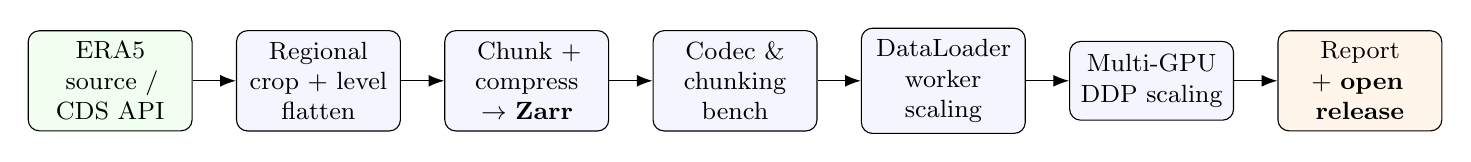
\begin{tikzpicture}[
  font=\small,
  box/.style={draw, rounded corners, align=center, inner sep=4pt,
              minimum height=10mm, text width=18mm, fill=blue!4},
  acc/.style={box, fill=green!6}, rel/.style={box, fill=orange!8},
  node distance=5.5mm]
\node[acc] (a) {ERA5 source / CDS API};
\node[box, right=of a] (b) {Regional crop + level flatten};
\node[box, right=of b] (c) {Chunk + compress \textbf{$\rightarrow$ Zarr}};
\node[box, right=of c] (d) {Codec \& chunking bench};
\node[box, right=of d] (e) {DataLoader worker scaling};
\node[box, right=of e] (f) {Multi-GPU DDP scaling};
\node[rel, right=of f] (g) {Report + \textbf{open release}};
\foreach \x/\y in {a/b,b/c,c/d,d/e,e/f,f/g} \draw[-{Latex[length=2mm]}] (\x) -- (\y);
\end{tikzpicture}
\caption{End-to-end pipeline. ERA5 is acquired and regionally cropped (or the
released store is downloaded directly), written as a chunked, compressed Zarr,
and benchmarked along the four parallel/distributed levers (codec, chunking,
DataLoader workers, DDP); results and the dataset itself are openly released.}
\label{fig:pipeline}
\end{figure*}

%------------------------------------------------------------------------------
\section{Background and Related Work}
\textbf{ERA5 and weather-ML data.} ERA5~\cite{era5} is the de facto training
source for ML weather models. Following WeatherBench2~\cite{wb2} and
FourCastNet~\cite{fcn} conventions, each pressure-level variable at a level
becomes its own 2-D channel (e.g.\ \texttt{z500}, \texttt{t850}), so the
dataset is a stack of $(\textrm{time},\textrm{lat},\textrm{lon})$ channels.
Two random-access patterns dominate training: (a) a \emph{full spatial field}
at one random time, used by CNN/diffusion models such as
StormCast~\cite{stormcast} and CorrDiff~\cite{corrdiff}; and (b) a \emph{full
time series} at one point, used by point-forecasting (e.g.\ LSTM) models. As
we show, the two favour opposite on-disk layouts.

\textbf{Zarr.} Zarr~\cite{zarr} stores an N-D array as a grid of
independently compressed chunk files plus JSON metadata. Two properties make
it attractive for parallel training: chunks are addressed directly by index
(random access without scanning), and each chunk is an independent compressed
object, so reads parallelize across processes with no shared state. We use
\texttt{zarr}$<$3 with numcodecs Blosc~\cite{blosc}, a meta-compressor that
applies a byte-\emph{shuffle} filter before LZ4 or Zstd.

\textbf{Dataset.} Our dataset is ERA5 obtained from the Copernicus Climate
Data Store (CDS) and regridded to a StormCast-style ``LowRes'' regional grid:
24 channels (surface \texttt{mslp}, \texttt{t2m}, \texttt{u10}, \texttt{v10},
plus \texttt{q,t,u,v,z} at 1000/850/500/250\,hPa) on a $224\times128$
curvilinear grid covering a $4.0^\circ\times2.5^\circ$ Taiwan box at
$\approx$2.0\,km spacing, hourly from 2019-08 to 2022-12: a 21\,216-step
training split (2019-08 to 2021-12) and an 8\,760-step validation split
(2022), 29\,976 hourly steps in total ($\approx$3.42\,yr), 82.5\,GB as
\texttt{float32}. Because each CDS request waits in a shared queue for minutes
to hours and can fail or stall, we package the assembled store for direct
download (Sec.~\ref{sec:release}). The codec/chunking/loader benchmarks use a
744-step (31-day) subset at the full $224\times128$ grid and all 24 channels:
the trade-offs we study are properties of the \emph{layout} and are relative
between configurations, while the full-horizon figures enter the storage
analysis. The subset is also operationally necessary --- the finest layout
alone writes 688\,188 chunk files, and a six-layout sweep of the full store
would exceed the shared node's free memory and inode budget.

%------------------------------------------------------------------------------
\section{Methodology}
The pipeline (Fig.~\ref{fig:pipeline}) acquires the data and then isolates
four parallel/distributed levers, one experiment each.

\textbf{Acquisition (parallel I/O).} Acquisition issues one CDS request per
$(\textrm{year},\textrm{month},\textrm{stream})$ concurrently through a thread
pool to hide per-request queue latency. We do not report acquisition time as a
benchmark: CDS queue latency is dominated by server-side load we neither
control nor can hold fixed --- that variability is precisely what the open
release removes.

\textbf{Lever 1: codec.} At a fixed chunk shape we sweep seven numcodecs
compressors (none, Blosc-LZ4, Blosc-Zstd at levels 3/5/9, raw Zstd, gzip).
All are \emph{lossless}: every store round-trips the \texttt{float32} fields
bit-exactly, so ``success'' is a smaller and/or faster-to-read store with
identical reconstruction.

\textbf{Lever 2: chunk shape.} At a fixed codec we sweep six
$(\textrm{time},\textrm{lat},\textrm{lon})$ chunk shapes, from
\texttt{full\_field} $(1,224,128)$ --- one timestep per chunk --- through
\texttt{daily}/\texttt{weekly}/\texttt{monthly} $(T,224,128)$ and
\texttt{spatial\_block} $(24,32,32)$ to \texttt{timeseries} $(744,1,1)$ ---
one grid point's entire series per chunk. For each we measure on-disk size,
chunk-file count, build time, and the throughput of \emph{both} dominant
access patterns.

\textbf{Lever 3: parallel loading.} A PyTorch~\cite{pytorch}
\texttt{Dataset} yields consecutive-frame samples $(x_t, x_{t+1})$; the Zarr
handle is re-opened in each worker process, so workers read and decompress
disjoint chunks with no shared state (embarrassingly parallel reads). We sweep
\texttt{num\_workers} $\in\{0,1,2,4,8\}$; 0 means loading in the training
process itself.

\textbf{Lever 4: data-parallel training.} A small convolutional forecaster is
trained under PyTorch DDP~\cite{ddp} (NCCL) with a
\texttt{DistributedSampler} sharding the time axis across ranks; we sweep
world size $\{1,2,3\}$ for a strong-scaling curve. Each step we time, with
CUDA synchronization, the phase blocked on data (next-batch wait plus
host-to-device copy) and the compute phase (forward/backward/optimizer,
including gradient all-reduce) separately.

\textbf{Metrics.} Fields/s and series/s denote random full-field and random
point-series reads per second; samples/s counts $(x_t,x_{t+1})$ training
pairs. For $p$ GPUs with aggregate throughput $X(p)$, speedup is
$S(p)=X(p)/X(1)$ and strong-scaling efficiency $E(p)=S(p)/p$. The
\emph{data-bound fraction} is
$f_{\mathrm{data}}=t_{\mathrm{data}}/(t_{\mathrm{data}}+t_{\mathrm{comp}})$,
summed over ranks and timed steps. \emph{Read amplification} is bytes read
from the store divided by bytes actually returned to the consumer.

%------------------------------------------------------------------------------
\section{Experimental Setup}
\textbf{Hardware.} One shared node (\texttt{gpu03}): dual-socket Intel Xeon
Gold 6226R (32 cores / 64 threads), 810\,GB RAM ($\approx$89\,GB free during
runs; the node is multi-user), 3$\times$ NVIDIA RTX~A6000 (48\,GB).
\textbf{Software.} Python 3.10.12; PyTorch 2.6.0+cu124 with NCCL; zarr 2.18.3;
numcodecs 0.13.1; xarray 2025.6.1; NumPy 2.0.2. \textbf{Storage.} The project
and the released store live on NFS. Transient benchmark stores are placed on
tmpfs (\texttt{/dev/shm}) to avoid the NFS small-file penalty (the
\texttt{timeseries} layout alone creates 688\,188 files); tmpfs numbers
therefore isolate chunk addressing and decompression from disk latency and are
upper bounds for disk-resident stores, while the DDP and released-store
experiments run against NFS.

\textbf{Measurement protocol.} Every phase is wall-clock timed; every metric
row is stamped with a hardware/software fingerprint and appended to CSV/JSONL
for full provenance. The RNG seed is fixed (1234). Random-access probes draw
64--128 frames/points per configuration, except the \texttt{timeseries}
field probe (6 frames), where a single field read touches the entire store
(Sec.~\ref{sec:disc}). The DataLoader benchmark times 40 batches of 32 after a
warm-up batch; DDP times 100 steps after 10 warm-up steps, batch 32 per rank,
4 loader workers. We report one run per configuration; as an indication of
run-to-run spread, the \texttt{full\_field}+\texttt{blosc\_zstd5} store is
independently rebuilt and re-probed by three different scripts, which agree to
$<$0.1\% in size and $\approx$5\% in write time and read latency. DDP on the
shared node is noisier: one world-size-2 run hit a transient NCCL stall under
GPU contention and was re-run; we report the least-contended run per world
size. Sizes use decimal units (1\,MB $=10^6$\,B).

%------------------------------------------------------------------------------
\section{Results}

\textbf{Storage footprint and global scale.}
Table~\ref{tab:size} gives the headline storage numbers. The 3.42-year
regional dataset is 82.5\,GB uncompressed --- the regional crop alone keeps
$28\,672/1\,038\,240 = 1/36$ of the $0.25^\circ$ global grid points. The
production Zarr compresses the benchmark subset $1.88\times$ losslessly
(2\,047.9\,MB $\rightarrow$ 1\,090.9\,MB at 61\,MB/s write), and the layouts
studied below reach up to $8.47\times$, i.e.\ 9.7--44\,GB for the full
horizon. Extrapolating the same horizon and channels to the globe gives
2.99\,TB at $0.25^\circ$ and 366.7\,TB (equal-area) to 534.7\,TB (grid
product) at this dataset's $\approx$2\,km resolution: the compressed regional
store is $68$--$307\times$ smaller than the global $0.25^\circ$ archive and
$\approx$$10^4\times$ smaller than a global 2\,km one.

\begin{table}[t]
\caption{Regional dataset vs.\ equivalent global stores over the same
3.42-yr hourly horizon and 24 \texttt{float32} channels.}
\label{tab:size}
\centering\small
\begin{tabular}{@{}lrr@{}}
\toprule
Scope & Grid points & Uncompressed \\
\midrule
Regional, $\approx$2\,km (this dataset) & $28\,672$ & 82.5\,GB \\
Global, $0.25^\circ$ (native ERA5) & $1.04$\,M & 2.99\,TB \\
Global, $\approx$2\,km (equal-area) & $127$\,M & 366.7\,TB \\
Global, $\approx$2\,km (grid product) & $186$\,M & 534.7\,TB \\
\bottomrule
\end{tabular}
\end{table}

\textbf{Codecs.}
Table~\ref{tab:codec} and Fig.~\ref{fig:codec} sweep codecs at fixed
\texttt{full\_field} chunking. \texttt{blosc\_zstd5} achieves the best ratio
($1.88\times$) while keeping random-frame reads at 5.9\,ms, and is adopted as
the default. Two effects dominate. First, Blosc's byte-shuffle filter is
decisive: at the same nominal compressor and level, \texttt{blosc\_zstd5}
reaches $1.88\times$ versus $1.25\times$ for raw \texttt{zstd5}, because
shuffling groups the slowly-varying \texttt{float32} exponent bytes. Second,
\texttt{gzip} is strictly dominated: a worse ratio than Blosc-Zstd
\emph{and} $3.7\times$ its random-frame latency (21.8 vs.\ 5.9\,ms).
Uncompressed reads are fastest (3.5\,ms) but double the store. Raising Zstd
to level 9 (with bit-shuffle) does not pay: the store is no smaller and reads
are $1.5\times$ slower.

\begin{table}[t]
\caption{Codec sweep at \texttt{full\_field} chunking (744-step subset,
2\,047.9\,MB uncompressed). Ratio is vs.\ raw \texttt{float32}; Write/Read are
whole-store rates in MB/s; Frame = one random timestep, all channels.
$^{\dagger}$\texttt{blosc\_zstd9} uses bit-shuffle; all other Blosc rows use
byte-shuffle.}
\label{tab:codec}
\centering\small
\setlength{\tabcolsep}{4pt}
\begin{tabular}{@{}lrrrrr@{}}
\toprule
Codec & MB & Ratio & Write & Read & Frame (ms) \\
\midrule
none        & 2047.9 & 1.00 & 78.6 & \textbf{668.6} & \textbf{3.47} \\
blosc\_lz4  & 1263.2 & 1.62 & 73.0 & 670.5 & 4.68 \\
blosc\_zstd3& 1097.1 & 1.87 & 66.9 & 530.0 & 6.09 \\
\textbf{blosc\_zstd5} & \textbf{1090.9} & \textbf{1.88} & 64.5 & 552.6 & 5.88 \\
blosc\_zstd9$^{\dagger}$ & 1100.9 & 1.86 & \textbf{88.4} & 380.3 & 8.84 \\
zstd5       & 1642.0 & 1.25 & 63.1 & 410.2 & 6.73 \\
gzip5       & 1586.2 & 1.29 & 55.8 & 135.2 & 21.80 \\
\bottomrule
\end{tabular}
\end{table}

\begin{figure}[t]
  \centering
  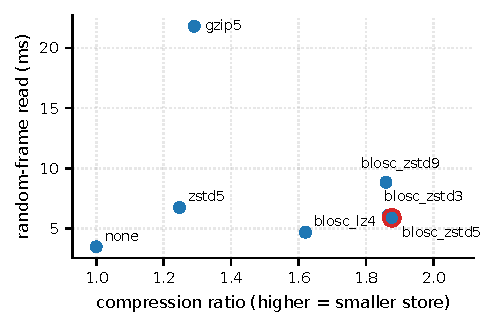
\includegraphics[width=0.92\columnwidth]{codecs.pdf}
  \caption{Codec trade-off at \texttt{full\_field} chunking: compression
  ratio vs.\ random-frame latency (lower right is better). The circled
  \texttt{blosc\_zstd5} sits on the Pareto frontier; \texttt{gzip5} is
  dominated on both axes.}
  \label{fig:codec}
\end{figure}

\textbf{Chunking --- the core trade-off.}
Table~\ref{tab:chunk} and Fig.~\ref{fig:chunk} quantify the central result.
\texttt{full\_field} delivers 170.6 random fields/s but only 0.42
point-series/s; \texttt{timeseries} inverts this to 181.2 series/s but 0.032
fields/s. Across layouts, random-field throughput therefore swings by a
factor of $5{,}300$ and series throughput by a factor of $430$ --- the chunk
shape is not a tuning detail but the dominant performance decision.
Compression \emph{improves} monotonically as more of the time axis enters
each chunk ($1.88\times\rightarrow3.58\times$ for
\texttt{full\_field}$\rightarrow$\texttt{monthly}), because consecutive hours
are highly correlated. \texttt{spatial\_block} $(24,32,32)$ is the balanced
choice: the \emph{best} compression ($8.47\times$ --- it adds spatial locality
within each chunk) while keeping both patterns usable (23.8 fields/s, 21.2
series/s). The extreme layouts also carry operational cost:
\texttt{timeseries} writes 688\,188 chunk files and took 942\,s to build,
$27\times$ longer than \texttt{spatial\_block} for the same bytes.

\begin{table}[t]
\caption{Chunk-shape sweep at \texttt{blosc\_zstd5} (744-step subset).
Fields/s = random full-field reads; series/s = random point-series reads.}
\label{tab:chunk}
\centering\small
\setlength{\tabcolsep}{3pt}
\begin{tabular}{@{}lrrrrr@{}}
\toprule
Chunking $(t,\textrm{lat},\textrm{lon})$ & \#files & MB & Ratio & fields/s & series/s \\
\midrule
full\_field $(1,224,128)$    & 17\,916 & 1090.9 & 1.88 & \textbf{170.6} & 0.42 \\
daily $(24,224,128)$         & 804     & 596.5  & 3.43 & 28.3 & 0.78 \\
weekly $(168,224,128)$       & 180     & 574.5  & 3.56 & 7.4  & 1.04 \\
monthly $(720,224,128)$      & 108     & 571.4  & 3.58 & 1.0  & 0.56 \\
spatial\_block $(24,32,32)$  & 20\,892 & \textbf{241.7} & \textbf{8.47} & 23.8 & 21.2 \\
timeseries $(744,1,1)$       & 688\,188& 365.8  & 5.60 & 0.032 & \textbf{181.2} \\
\bottomrule
\end{tabular}
\end{table}

\begin{figure}[t]
  \centering
  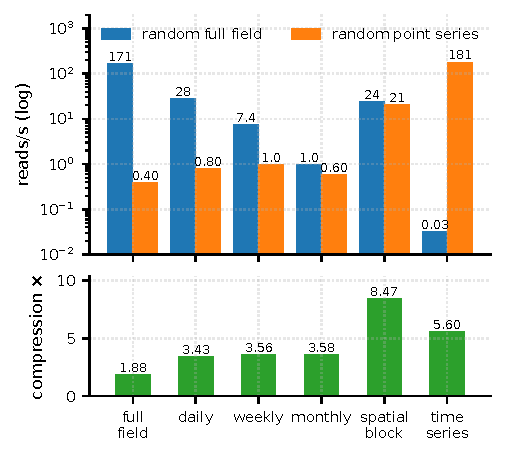
\includegraphics[width=0.96\columnwidth]{chunking.pdf}
  \caption{Chunk-shape trade-off. Top: random full-field vs.\ point-series
  throughput (log scale) --- \texttt{full\_field} and \texttt{timeseries} sit
  $5{,}300\times$ and $430\times$ apart on the two patterns;
  \texttt{spatial\_block} is the only layout fast on both. Bottom: lossless
  compression ratio of the same stores.}
  \label{fig:chunk}
\end{figure}

\textbf{DataLoader worker scaling.}
Fig.~\ref{fig:dl} shows training-sample throughput versus worker count
(per-layout values in Appendix~\ref{app:dl}). With \texttt{full\_field}
chunks, throughput rises from 74.4 samples/s in-process to 453.3 samples/s
with 8 workers ($6.1\times$); measured against the 1-worker rate the scaling
is $7.5\times$ over 8 workers, i.e.\ within 7\% of linear, with 56 of the 64
hardware threads still idle. Each random sample maps to exactly one chunk per
channel, so worker processes decompress disjoint chunks independently --- the
reads are embarrassingly parallel. Coarser temporal chunks suffer \emph{read
amplification}: a random single-frame sample must decompress an entire 24- or
168-step chunk and discard the rest, so \texttt{daily} peaks at 97.2 and
\texttt{weekly} at 16.3 samples/s. Workers still parallelize the (amplified)
decompression --- $7.1\times$ and $4.4\times$ at 8 workers --- but cannot
recover the $28\times$ base-rate gap. The dip from 0 to 1 worker (74.4
$\rightarrow$ 60.7) is the fixed cost of moving from in-process reads to one
worker process plus IPC; parallelism overtakes it from 2 workers on.

\begin{figure}[t]
  \centering
  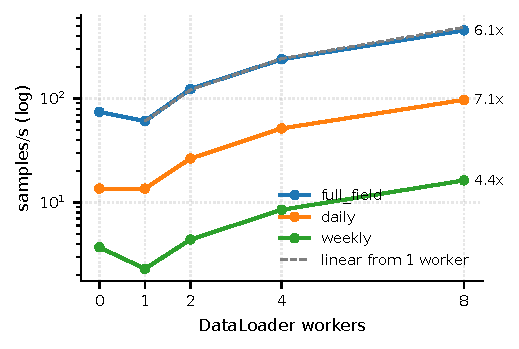
\includegraphics[width=0.96\columnwidth]{dataloader.pdf}
  \caption{PyTorch DataLoader throughput vs.\ \texttt{num\_workers} (log
  scale), annotated with each layout's 8-worker speedup over 0 workers.
  \texttt{full\_field} tracks the linear-from-1-worker reference (dashed)
  within 7\%; time-bundled layouts scale similarly but from a read-amplified,
  $7$--$28\times$ lower base.}
  \label{fig:dl}
\end{figure}

\textbf{Loading the released store in its native layout.}
The released dataset ships in its archival $(1326,3,28,16)$ chunking --- deep
in time, tiled in space. This is efficient for bulk temporal extraction but
pathological for random-frame training: one frame intersects all
$8\times8\times8=512$ channel/spatial chunks of its time block, so Zarr reads
$\approx$3.6\,GB to return a 2.75\,MB frame --- $1{,}326\times$ read
amplification, the time-depth of the chunk. A standalone DataLoader over this
store on NFS (Appendix~\ref{app:loader}) confirms the consequence: 0.026
random samples/s ($<$0.1\,MB/s useful payload while physically reading
94--124\,MB/s from NFS), essentially unchanged by adding workers because NFS
bandwidth, not CPU, is the limit; even chunk-aligned sequential access reaches
only 0.40 samples/s. Rechunking the \emph{same bytes} once to
\texttt{full\_field} raises random-frame loading to 74--453 samples/s
(Fig.~\ref{fig:dl}), a $10^3$--$10^4\times$ improvement. The release therefore
ships with our rechunking tool, and we recommend one rechunking pass (or
distribution directly in \texttt{full\_field}/\texttt{spatial\_block}) before
training.

\textbf{DDP strong scaling.}
Fig.~\ref{fig:ddp} reports end-to-end training throughput for 1--3 GPUs over
the NFS-resident \texttt{full\_field} production store. Global throughput
rises $125.0\rightarrow229.8\rightarrow297.9$ samples/s --- speedups
$1.00/1.84/2.38$, strong-scaling efficiencies $100/92/79\%$ --- while per-GPU
throughput falls $125.0\rightarrow99.3$ samples/s
(Appendix~\ref{app:ddp}). The data-bound fraction explains the erosion: it
stays at $0.80$--$0.82$ at every world size, so even this deliberately small
model spends $\approx$80\% of each step blocked on data, and every added GPU
multiplies random-read load on the same shared store. The NFS store is itself
the slow resource: inside training, rank~0 receives $\approx$125 samples/s
from it, about half of what the identical 4-worker loader draws from a
tmpfs-resident copy (238.9 samples/s, Fig.~\ref{fig:dl}). Compute-side cost
is secondary but visible: per-step compute (including gradient all-reduce)
grows from 47 to 64\,ms from 1 to 3 GPUs.

\begin{figure}[t]
  \centering
  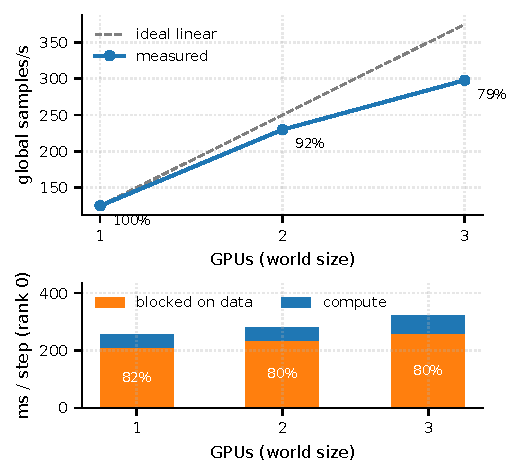
\includegraphics[width=0.96\columnwidth]{ddp_scaling.pdf}
  \caption{DDP strong scaling on 1--3 RTX~A6000 over the NFS
  \texttt{full\_field} store. Top: global throughput vs.\ the linear ideal,
  annotated with efficiency. Bottom: per-step time split on rank 0 --- the
  pipeline stays $\approx$80\% blocked on data at every world size, so GPUs
  are added to an already storage-limited pipeline.}
  \label{fig:ddp}
\end{figure}

%------------------------------------------------------------------------------
\section{Discussion and Analysis}\label{sec:disc}
\textbf{Why time-bundled chunks compress better yet read fields slower.}
Atmospheric fields are smooth in time: consecutive hourly frames are nearly
identical, so a chunk holding many timesteps lets shuffle+Zstd exploit
temporal redundancy ($1.88\times\rightarrow8.47\times$). But the
StormCast-style access pattern is ``one timestep, all channels'': with
\texttt{full\_field} that is exactly one chunk per channel, while a $T$-step
chunk forces decompressing and discarding $T{-}1$ unwanted frames --- read
amplification equal to the chunk's time depth (24 for \texttt{daily}, 1\,326
for the archival layout). The same temporal correlation that helps
compression hurts random-field latency: \emph{the most compressible layout is
the slowest for the target workload}. \texttt{timeseries} is the limit case:
one field read touches all $224\times128$ chunks of every channel
($\approx$688\,k chunk reads), hence 0.032 fields/s and our reduced probe
count there. \texttt{spatial\_block} escapes the trade-off because it adds a
\emph{second} locality axis: it bundles 24 hours for compression but tiles
space so a point series touches only its own $32\times32$ tiles, keeping the
two patterns within 12\% of each other (23.8 vs.\ 21.2 reads/s).

\textbf{Why reads scale with workers, and why DDP is data-bound.} Each chunk
is an independent compressed object and each worker holds its own store
handle, so decompression parallelizes with no coordination --- hence
near-linear (93\%) scaling to 8 workers on tmpfs. The DDP experiment then
localizes the training bottleneck: at $f_{\mathrm{data}}\approx0.8$ on an
NFS-resident store, three GPUs simply demand $3\times$ the random-read
bandwidth of one shared filesystem, and per-GPU throughput drops 21\%. The
actionable conclusion is that, at this model size, money and effort go to
\emph{storage, not GPUs}: more loader workers, staging the store to local
NVMe/tmpfs, or a prefetch-friendly layout each attack the 80\% of step time
spent waiting, whereas a fourth GPU attacks the other 20\%. A
production-scale model shifts the balance back toward compute; our
measurement marks where that crossover sits for this store.

\textbf{Choosing a layout.} For CNN/diffusion-style regional training,
\texttt{full\_field}+\texttt{blosc\_zstd5} maximizes feed throughput (170.6
fields/s; 453.3 samples/s at 8 workers) at the weakest compression. Where
storage or transfer is binding, \texttt{spatial\_block} stores $4.5\times$
less while both access patterns stay usable. \texttt{timeseries} should be
reserved for genuinely point-wise workloads: it is unusable for field access
and its 688\,188-file footprint is an inode/metadata liability on networked
filesystems (it also took $27\times$ longer to write).

\textbf{Limitations.} (i)~We report single runs; the $\approx$5\% spread we
measured across independent rebuilds of one configuration bounds timer noise
but not scheduler interference on the shared node, so DDP figures are
indicative rather than tightly controlled. (ii)~Layout benchmarks use one
month at full spatial resolution; relative trade-offs are layout-intrinsic,
but absolute rates depend on dataset size and page-cache state, and the
tmpfs-resident benchmarks bound disk-resident performance from above.
(iii)~The global 2\,km figures are an order-of-magnitude extrapolation
bracketed by the equal-area and grid-product constructions on a curvilinear
grid. (iv)~We deliberately use a small model, which overstates the data-bound
fraction relative to production models; quantifying the data/compute
crossover for a full-size StormCast network is future work. (v)~We do not
benchmark CDS acquisition itself, whose queue latency is not a controlled
quantity.

%------------------------------------------------------------------------------
\section{Open Dataset Release}\label{sec:release}
The most immediately reusable output of this work is the dataset itself: the
3.42-year, 24-channel, $\approx$2\,km Taiwan ERA5 store, regionally cropped,
channel-selected, and analysis-ready. Reassembling it from the CDS means
hours-to-days of queued, failure-prone requests behind a multi-terabyte
global archive; downloading it is a one-time 9.7--44\,GB transfer (layout
dependent), after which a regional StormCast/CorrDiff-style model trains on
it out of the box in the \texttt{full\_field} layout. The release includes
the Zarr store, the full benchmark/rechunking toolkit, per-result
hardware fingerprints, and every metric row behind the tables and figures in
this paper.\footnote{Download link and checksums are published in the project
repository README alongside the code, configuration, and raw metric logs.}

%------------------------------------------------------------------------------
\section{Conclusion}
A regional crop plus a chunked, compressed Zarr store turns a 3--535\,TB
(global) problem into a 9.7--44\,GB asset, and one knob dominates everything
downstream: the chunk shape. On identical data it moves lossless compression
from $1.88\times$ to $8.47\times$, swings the two training-relevant access
patterns by $5{,}300\times$ and $430\times$ in opposite directions, and
separates a store that feeds 453 samples/s from one that starves at 0.03.
For StormCast-style training, \texttt{full\_field} chunks scale to $6.1\times$
over 8 loader workers and keep three DDP GPUs at 79\% strong-scaling
efficiency --- yet the pipeline remains $\approx$80\% data-bound, so the next
dollar belongs to storage, not a fourth GPU. We release the analysis-ready
82.5\,GB Taiwan store with the complete, fingerprinted benchmark toolkit, so
the community can start from a ready-to-train artifact instead of the CDS
queue.

%------------------------------------------------------------------------------
\begin{thebibliography}{00}
\bibitem{fcn} J. Pathak \emph{et al.}, ``FourCastNet: A global data-driven
high-resolution weather model using adaptive Fourier neural operators,''
arXiv:2202.11214, 2022.
\bibitem{corrdiff} M. Mardani \emph{et al.}, ``Residual corrective diffusion
modeling for km-scale atmospheric downscaling (CorrDiff),'' arXiv:2309.15214,
2023.
\bibitem{stormcast} J. Pathak \emph{et al.}, ``Kilometer-scale convection
allowing model emulation using generative diffusion modeling (StormCast),''
arXiv:2408.10958, 2024.
\bibitem{era5} H. Hersbach \emph{et al.}, ``The ERA5 global reanalysis,''
\emph{Q. J. R. Meteorol. Soc.}, vol.~146, no.~730, pp.~1999--2049, 2020.
\bibitem{wb2} S. Rasp \emph{et al.}, ``WeatherBench 2: A benchmark for the
next generation of data-driven global weather models,'' \emph{J. Adv. Model.
Earth Syst.}, vol.~16, 2024.
\bibitem{zarr} A. Miles \emph{et al.}, ``Zarr: chunked, compressed,
N-dimensional arrays,'' software, \url{https://zarr.dev}, 2024.
\bibitem{blosc} F. Alted, ``Why modern CPUs are starving and what can be done
about it,'' \emph{Comput. Sci. Eng.}, vol.~12, no.~2, pp.~68--71, 2010
(Blosc).
\bibitem{pytorch} A. Paszke \emph{et al.}, ``PyTorch: An imperative style,
high-performance deep learning library,'' in \emph{NeurIPS}, 2019.
\bibitem{ddp} S. Li \emph{et al.}, ``PyTorch Distributed: Experiences on
accelerating data parallel training,'' \emph{Proc. VLDB Endow.}, vol.~13,
no.~12, 2020.
\end{thebibliography}

% ---- end of main body + references; Appendix below is NOT counted. ----
\xdef\mainbodyendpage{\thepage}

%==============================================================================
%  APPENDIX (Category A: optional -- extra data and reproduction details)
%==============================================================================
\appendices

\section{Reproduction}
From the repository root (\texttt{.venv} active), the full benchmark is:
\begin{lstlisting}
# bridge the StormCast LowRes store -> size report + 1-month subset
python scripts/90_ingest_stormcast.py --src <LowRes> --steps 744
python scripts/03_build_zarr.py            # production Zarr + footprint
python scripts/04_bench_codecs.py          # codec sweep
python scripts/05_bench_chunking.py --keep # 6 chunkings (keeps stores)
python scripts/06_bench_dataloader.py \
       --strategies full_field daily weekly
for ws in 1 2 3; do torchrun --standalone \
   --nproc_per_node=$ws scripts/07_bench_ddp.py; done
# loading speed of the RELEASED store in its native layout
python scripts/09_bench_lowres_loader.py --src <LowRes> \
       --access random --workers 0 2
python scripts/08_report.py --plots        # tables + figures (png+pdf)
\end{lstlisting}
Each script appends a fingerprinted row to \texttt{results/<name>.\{csv,jsonl\}};
\texttt{results/dataset\_size\_report.json} holds the size/global computation.

\section{DataLoader Scaling Detail}\label{app:dl}
Samples/s vs.\ \texttt{num\_workers} (batch 32, 40 timed batches, 2-frame
window, \texttt{blosc\_zstd5}, tmpfs stores); right column: 8-worker speedup
over 0 workers.
\begin{center}\small
\begin{tabular}{@{}lrrrrrr@{}}
\toprule
chunking & 0 & 1 & 2 & 4 & 8 & speedup \\
\midrule
full\_field & 74.4 & 60.7 & 123.8 & 238.9 & 453.3 & $6.1\times$ \\
daily       & 13.6 & 13.6 & 26.5  & 51.6  & 97.2  & $7.1\times$ \\
weekly      & 3.7  & 2.3  & 4.4   & 8.5   & 16.3  & $4.4\times$ \\
\bottomrule
\end{tabular}
\end{center}

\section{DDP Strong-Scaling Detail}\label{app:ddp}
NCCL backend, NFS-resident \texttt{full\_field} store, batch 32 per rank, 4
loader workers, 100 timed steps after 10 warm-up steps. Times are per-step
averages on rank 0.
\begin{center}\small
\setlength{\tabcolsep}{3.5pt}
\begin{tabular}{@{}rrrrrrr@{}}
\toprule
GPUs & glob.\ s/s & per-GPU & $S(p)$ & $E(p)$ & $f_{\mathrm{data}}$ & data/comp (ms) \\
\midrule
1 & 125.0 & 125.0 & 1.00 & 100\% & 0.82 & 209 / 47 \\
2 & 229.8 & 114.9 & 1.84 & 92\%  & 0.80 & 234 / 44 \\
3 & 297.9 & 99.3  & 2.38 & 79\%  & 0.81 & 258 / 64 \\
\bottomrule
\end{tabular}
\end{center}

\section{Released-Store Native-Layout Loader}\label{app:loader}
DataLoader throughput reading the released LowRes Zarr on NFS in its native
$(1326,3,28,16)$ chunking (read amplification $1{,}326\times$; eff.\ = useful
frame bytes/s, phys.\ = bytes actually read/s).
\begin{center}\small
\begin{tabular}{@{}llrrr@{}}
\toprule
access & workers & samples/s & eff.\ MB/s & phys.\ MB/s \\
\midrule
random     & 0 & 0.026 & 0.1 & 93.6 \\
random     & 2 & 0.034 & 0.1 & 124.0 \\
sequential & 0 & 0.173 & 0.5 & 631.6 \\
sequential & 2 & 0.404 & 1.1 & 1473.3 \\
\bottomrule
\end{tabular}
\end{center}
For comparison, the rechunked \texttt{full\_field} store
(Appendix~\ref{app:dl}) reaches 74--453 samples/s on the same access pattern.

\end{document}
